\documentclass[9pt]{beamer}

\usepackage{beamerpreamble}
\usepackage[swedish]{babel}
\usepackage{minted}
\usepackage{comment}
\usemintedstyle{vs}
\usepackage{xcolor}
\usepackage{tikz}
\usepackage{textgreek}
\usepackage{dirtytalk}

\renewcommand{\ttdefault}{cmtt}

\newcommand*\mean[1]{\bar{#1}}

\title{Datalaboration - Förberedande tutorial}
\author[benjamin.eriksson@physics.uu.se]{Benjamin Eriksson  \\ \tiny{med inspiration från} \\ \scriptsize{Slides av M. Isacson, M. Ellert, M. Olvegård, och B. Lindgren}}
\institute[Uppsala universitet]{{\small Avdelningen för tillämpad kärnfysik \\ Institutionen för fysik och astronomi} \\ \uulogo}
\date{{\small Reviderad}\\ \today}

\begin{document}
    \begin{frame}{Mätvärdesbehandling}
        Efter denna föreläsning ska du kunna beräkna
        \begin{enumerate}
            \item medelvärden
            \item standardavvikelser
            \item standardosäkerheten hos ett medelvärde
        \end{enumerate}
        \vspace{0.5cm}
        samt veta
        \begin{itemize}
            \item hur man presenterar mätosäkerheter
            \item hur många värdesiffror man bör ange
        \end{itemize}
    \end{frame}
    
    \begin{frame}{Medelvärde, standardavvikelse \& standardosäkerhet}
        \onslide<+->
        Säg att ni från slumpvariabeln $X$ erhållit mätserien $\{x_i\}_1^n$. Viktiga frågor är då
        
        \begin{enumerate}
            \item Vad är det förväntade värdet för en mätning $x_i$?
            \item Hur stor är spridningen hos mätvärdena?
            \item Hur väl kan vi skatta det sanna väntevärdet av slumpvariabeln $X$?
        \end{enumerate}

        \vfill

        \begin{columns}[T]
        \column{.6\textwidth}
        
            \begin{enumerate}
                \item<+-> Medelvärdet: $\mean{x} = \frac1n \sum\limits_{i=1}^n x_i$
                    \begin{itemize}
                        \item $\mean{x}$ skattar väntevärdet $\mu=E[x]$.
                    \end{itemize}
                \item<+-> Standardavvikelse: \\
                    \vspace{0.5em}
                    $u(x) = \sqrt{\frac1{n-1} \sum\limits_{i=1}^n \left(x_i - \mean{x}\right)^2}$
                    \vspace{0.5em}
                    \begin{itemize}
                        \item $u(x)$ är ett mått på spridningen av mätvärdena $x_i$ och skattar den sanna standardavvikelsen $\sigma$.
                    \end{itemize}
                \item<+-> Standardosäkerhet i medelvärdet: \\
                    \vspace{0.5em}
                    $u(\mean{x}) = \frac{u(x)}{\sqrt{n}} = \sqrt{\frac1{n(n-1)} \sum_{i=1}^n \left(x_i - \mean{x}\right)^2}$
                    \vspace{0.5em}
                    \begin{itemize}
                        \item $u(\mean{x})$ skattar \emph{spridningen i medelvärdet} vi skulle få om experimentet upprepades flera gånger.
                    \end{itemize}
            \end{enumerate}
            
            \column{.4\textwidth}
            \hspace{-0.2\textwidth}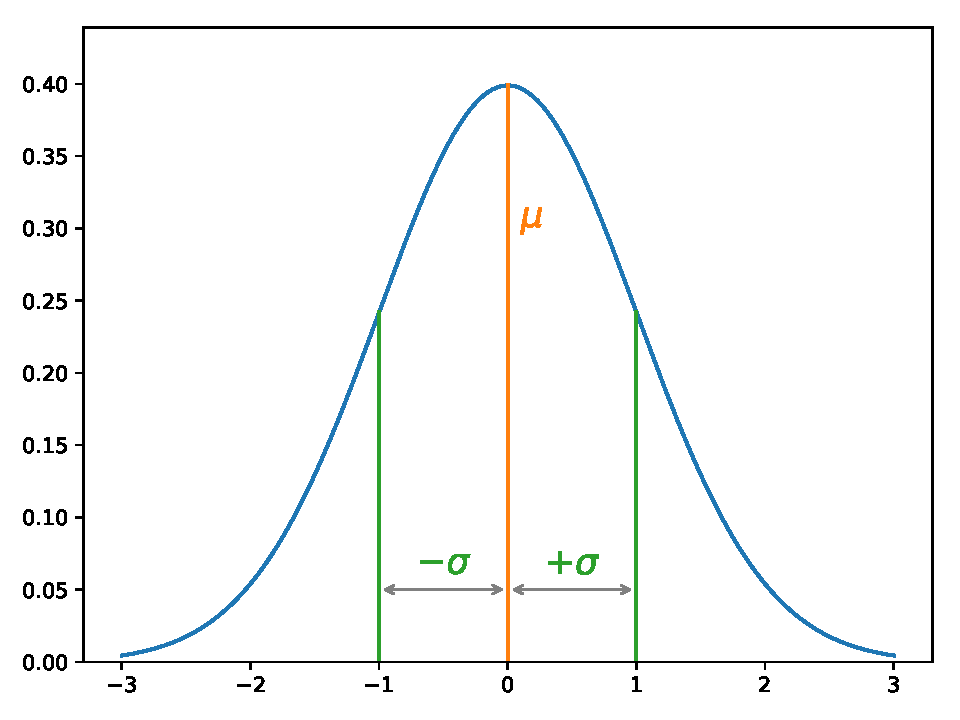
\includegraphics[width=1.2\textwidth]{gaus.pdf}
        \end{columns}
        
    \end{frame}

    \begin{frame}[t]{Exempel}
        Låt $x = [0.97, 1.09, 1.16, 1.04, 1.12]$. Medelvärdet är då
        \begin{equation*}
            \bar{x} = \frac{1}{n}\sum\limits_{i=1}^n x_i = \frac{0.97+1.09+1.16+1.04+1.12}{5} = 1.08
        \end{equation*}
        
        Beräkna standardavvikelsen
        \begin{equation*}
            u(x) = \sqrt{\frac1{n-1} \sum\limits_{i=1}^n \left(x_i - \mean{x}\right)^2}
        \end{equation*}
        och standardosäkerheten i medelvärdet
        \begin{equation*}
            u(\mean{x}) = \frac{u(x)}{\sqrt{n}} = \sqrt{\frac1{n(n-1)} \sum_{i=1}^n \left(x_i - \mean{x}\right)^2}
        \end{equation*}
        
        \vspace{0.5cm}
        \begin{center}
            \textcolor{red}{Ange svaret i fältet till höger om föreläsningen i Studium!}    
        \end{center}
        
        
    \end{frame}
    
    \begin{frame}[t]
    Obligatoriskt:
    \begin{itemize}
        \item Öppna \textit{tutorial\_2.mlx} och gör sektionen som heter \textcolor{orange}{Tutorial 2 - Mätvärdesbehandling}.
    \end{itemize}
    \vspace{1cm}
    Beskriv i ord vad skillnaden är mellan \textit{standardavvikelse} och \textit{standardosäkerheten hos ett medelvärde} i rutan till höger om föreläsningen i Studium!
    \end{frame}
    
    \begin{frame}{Hur presenteras osäkerheter?}
        \hrule\vspace{0.6em}
        \textcolor{red}{\textbf{Scenario}}\\ 
        Vi har mätt mängden arsenik i nederbörden i Uppsala varje månad under 2018 (givet som \textmu g arsenik per liter regn) och beräknat
        \begin{itemize}
            \item medelvärde från året: $\bar{x} = 0.1109$ \textmu g/l
            \item standardosäkerheten hos medelvärdet: $u\left(\bar{x}\right) = 0.025647$ \textmu g/l
        \end{itemize}
        \vspace{0.6em}\hrule
        \pause
        \begin{block}{Tumregel}
            Avrunda osäkerheten till \textbf{två värdesiffror} och justera mätetalet därefter.
        \end{block}
        \vspace{0.2cm}
        Vi får då $u(\bar{x}) = 0.026$ \textmu g/l och därmed $\bar{x} = 0.111$ \textmu g/l.
        \vspace{0.5cm}
        
        \pause
        Två godkända sätt att presentera osäkerheten:
        \begin{equation*}
            \mean{x} = \num[separate-uncertainty=true]{0.111 \pm 0.026} \text{ \textmu g/l} 
            \quad
            \text{eller}
            \quad
            \mean{x} = \num{0.111 \pm 0.026} \text{ \textmu g/l}   
        \end{equation*}
        
        
        
        \begin{equation*}
            \left(0.085 < \bar{x} < 0.137\right)
        \end{equation*}
            
    \end{frame}
    

\end{document}